\documentclass[article,12pt]{elsarticle}
\usepackage[utf8]{inputenc}
\usepackage{graphicx}
\usepackage{booktabs}
\usepackage{subcaption}
\usepackage{amssymb}
\usepackage{flushend}
\usepackage{float}
\usepackage{amsmath}
\usepackage{amsfonts}
\usepackage{dcolumn}
\usepackage{amsthm}
\usepackage{caption}
\usepackage{lmodern}
\usepackage{booktabs}
\usepackage{color}
\usepackage{longtable}
\usepackage{rotating}
\usepackage{etoolbox}
\usepackage{hyperref}
\usepackage{comment}
\usepackage{pdflscape}
\usepackage{comment}
\usepackage[table,xcdraw]{xcolor}
\usepackage[framemethod=TikZ]{mdframed}
\usepackage[a4paper, left=1.5cm, right=1.5cm, top=2cm, bottom=2cm]{geometry}

\begin{document}

\mdfsetup{innertopmargin=10pt,linecolor=blue!20,%
linewidth=2pt,topline=true,
frametitleaboveskip=\dimexpr-\ht\strutbox\relax,}

\begin{frontmatter}
    \title{Laboratorio de Óptica \\  Práctica  II: Reflexión y Refracción}
    \author{López González Andrés$^1$, Reyes Saldivar Ailton Uriel$^2$ y Gante Morales Pedro José$^3$} %Aquí va el nombre de los integrantes que participaron en el informe.
    \address{$^1$ Facultad de Ciencias, Universidad Nacional Autónoma de México, M\'exico CDMX.}

\begin{abstract}
Se estudia la reflexión y refracción de un haz láser en la interfaz aire-acrílico y acrílico-aire para verificar la Ley de Reflexión y la Ley de Snell. Se determina el índice de refracción del acrílico por dos métodos: ajuste de datos experimentales ($n = 1.5052 \pm 0.0650$) y medición del ángulo crítico ($n = 1.4665 \pm 0.3925$). Además, se calcula la velocidad de la luz en el acrílico, obteniendo $(2.027 \pm 0.194) \times 10^8$ m/s. Se cuantifica la incertidumbre mediante propagación de errores y se identifican las principales fuentes de error en la medición angular. Los resultados confirman la validez de la óptica geométrica y resaltan la importancia de minimizar errores sistemáticos en mediciones de alta precisión.
\end{abstract}
    
\end{frontmatter}

\vspace{0.5cm} 

\section{Introducción}

\subsection*{Óptica Geométrica}
La óptica geométrica es una aproximación en la que la luz se modela como un conjunto de rayos ideales que se propagan en línea recta dentro de un medio homogéneo y transparente. Este enfoque es válido cuando la longitud de onda de la luz es pequeña en comparación con los objetos con los que interactúa. En este contexto, los cambios en la dirección de propagación de la luz pueden explicarse mediante las leyes de reflexión y refracción \cite{Pedrotti2018}.

\subsection*{Principio de Fermat}
El principio de Fermat establece que el trayecto seguido por un rayo de luz entre dos puntos es aquel que minimiza o hace estacionario el tiempo de recorrido. Este principio es una consecuencia del comportamiento ondulatorio de la luz y puede ser utilizado para derivar las leyes fundamentales de la óptica geométrica \cite{Hecht2000, Pedrotti2018}.

\subsection*{Ley de Reflexión}
Cuando un rayo de luz incide sobre una superficie reflectante, se observa que el ángulo de incidencia $\theta_I$ es igual al ángulo de reflexión $\theta_R$:

\begin{mdframed}
\begin{equation}
\theta_I = \theta_R
\end{equation}
\end{mdframed}

Esta ecuación indica que el rayo reflejado se encuentra en el mismo plano que el rayo incidente y la normal a la superficie en el punto de incidencia. Dependiendo de la naturaleza de la superficie, la reflexión puede ser especular (si la superficie es lisa) o difusa (si la superficie es rugosa) \cite{Hecht2000, Tipler1999}.

\subsection*{Linealización de la Ley de Reflexión}
Podemos expresar la ecuación en una forma lineal tipo $y = mx + b$:

\begin{mdframed}
\begin{equation}
\theta_R = 1 \cdot \theta_I + 0
\end{equation}
\end{mdframed}

Definiendo las variables:
\begin{itemize}
\item $x' = \theta_I$
\item $y' = \theta_R$
\item Pendiente: $m = 1$
\item Intersección con el eje: $b = 0$
\end{itemize}

Para comprobar experimentalmente la Ley de Reflexión, se espera que:
\begin{equation}
m = 1, \quad b = 0
\end{equation}

\subsection*{Ley de Refracción (Ley de Snell)}
Cuando un rayo de luz atraviesa la interfaz entre dos medios con índices de refracción distintos, cambia su dirección según la relación:

\begin{mdframed}
\begin{equation}
\frac{\sin \theta_I}{\sin \theta_T} = \frac{v_I}{v_T} = \frac{n_T}{n_I}
\end{equation}
\end{mdframed}

\subsection*{Linealización de la Ley de Snell}
Reescribimos la ecuación en forma lineal $y = mx + b$:

\begin{mdframed}
\begin{equation}
\sin \theta_T = \left( \frac{v_I}{v_T} \right) \sin \theta_I + 0
\end{equation}
\end{mdframed}

Definiendo:
\begin{itemize}
\item $y' = \sin \theta_T$
\item $x' = \sin \theta_I$
\item Pendiente: $m = \frac{v_I}{v_T}$
\item Intersección con el eje: $b = 0$
\end{itemize}

De esta forma, el ajuste de datos experimentales a una línea recta permite determinar el cociente de los índices de refracción de los dos medios involucrados.

\subsection*{Determinación del Índice de Refracción mediante el Ángulo Crítico}
El índice de refracción ($n$) de un material puede determinarse midiendo el \textbf{ángulo crítico de reflexión interna total} ($\theta_c$) cuando la luz pasa de un medio más denso (con índice de refracción $n$) a un medio menos denso (como el aire, con índice de refracción $n_{\text{aire}} \approx 1$). La relación entre el ángulo crítico y el índice de refracción está dada por la Ley de Snell:
\begin{mdframed}
\begin{equation}
n \cdot \sin(\theta_c) = n_{\text{aire}} \cdot \sin(90^\circ)
\end{equation}
\end{mdframed}

Dado que $\sin(90^\circ) = 1$, la ecuación se simplifica a:

\begin{mdframed}
\begin{equation}
n = \frac{1}{\sin(\theta_c)}
\end{equation}
\end{mdframed}

Por lo tanto, si medimos el ángulo crítico $\theta_c$, podemos calcular el índice de refracción $n$ del material.




\subsection{Hipótesis}

Si la luz incide sobre una interfaz entre dos medios con distintos índices de refracción, entonces su comportamiento seguirá las leyes de reflexión y refracción establecidas en la óptica geométrica. En particular:
\begin{itemize}
\item La relación entre los ángulos de incidencia y reflexión confirmará que $\theta_I = \theta_R$.
\item La ecuación de Snell permitirá calcular la velocidad de la luz en el acrílico a partir de la medición de los ángulos de incidencia y refracción.
\item La determinación del ángulo crítico permitirá obtener el índice de refracción del acrílico, verificando que coincide con valores teóricos esperados.
\end{itemize}



\subsection{Objetivos}

\begin{enumerate}

\item Medir los ángulos de incidencia y reflexión en la cara plana del acrílico para verificar la Ley de Reflexión.
\item Medir los ángulos de incidencia y refracción en la cara plana del acrílico para verificar la Ley de Snell.
\item Repetir la medición de los ángulos en la cara circular del acrílico y analizar su efecto en la refracción de la luz.
\item Determinar la velocidad de la luz en el acrílico utilizando la relación establecida por la Ley de Snell.
\item Medir el ángulo crítico de reflexión interna total para calcular el índice de refracción del acrílico.
\item Evaluar la propagación de incertidumbres en la determinación del índice de refracción y la velocidad de la luz en el material.
\end{enumerate}





\section{Desarrollo Experimental}

\subsection{Primera parte: Incidencia en la cara plana (Aire-Acrílico)}
Para la primera parte del experimento, se hizo incidir un haz de luz láser en la cara plana del bloque de acrílico. Se midieron los ángulos de incidencia, reflexión y refracción utilizando un goniómetro con el objetivo de verificar la Ley de Reflexión y la Ley de Snell.

Las medidas de los ángulos incidentes se realizaron en incrementos de $5^\circ$, midiendo los ángulos de reflexión y refracción respecto a la normal de la superficie plana. Se observó que, inicialmente, el ángulo refractado aumentaba en intervalos de aproximadamente $3^\circ$ a $3.5^\circ$. A partir de $50^\circ$, el ángulo refractado comenzó a aumentar en incrementos de $2^\circ$. Cuando el ángulo de incidencia alcanzó los $80^\circ$, el láser dejó de comportarse como un haz colimado y se dispersó, lo que generó una incertidumbre de definición de aproximadamente $\pm 2^\circ$.

\begin{figure}[H]
    \centering
    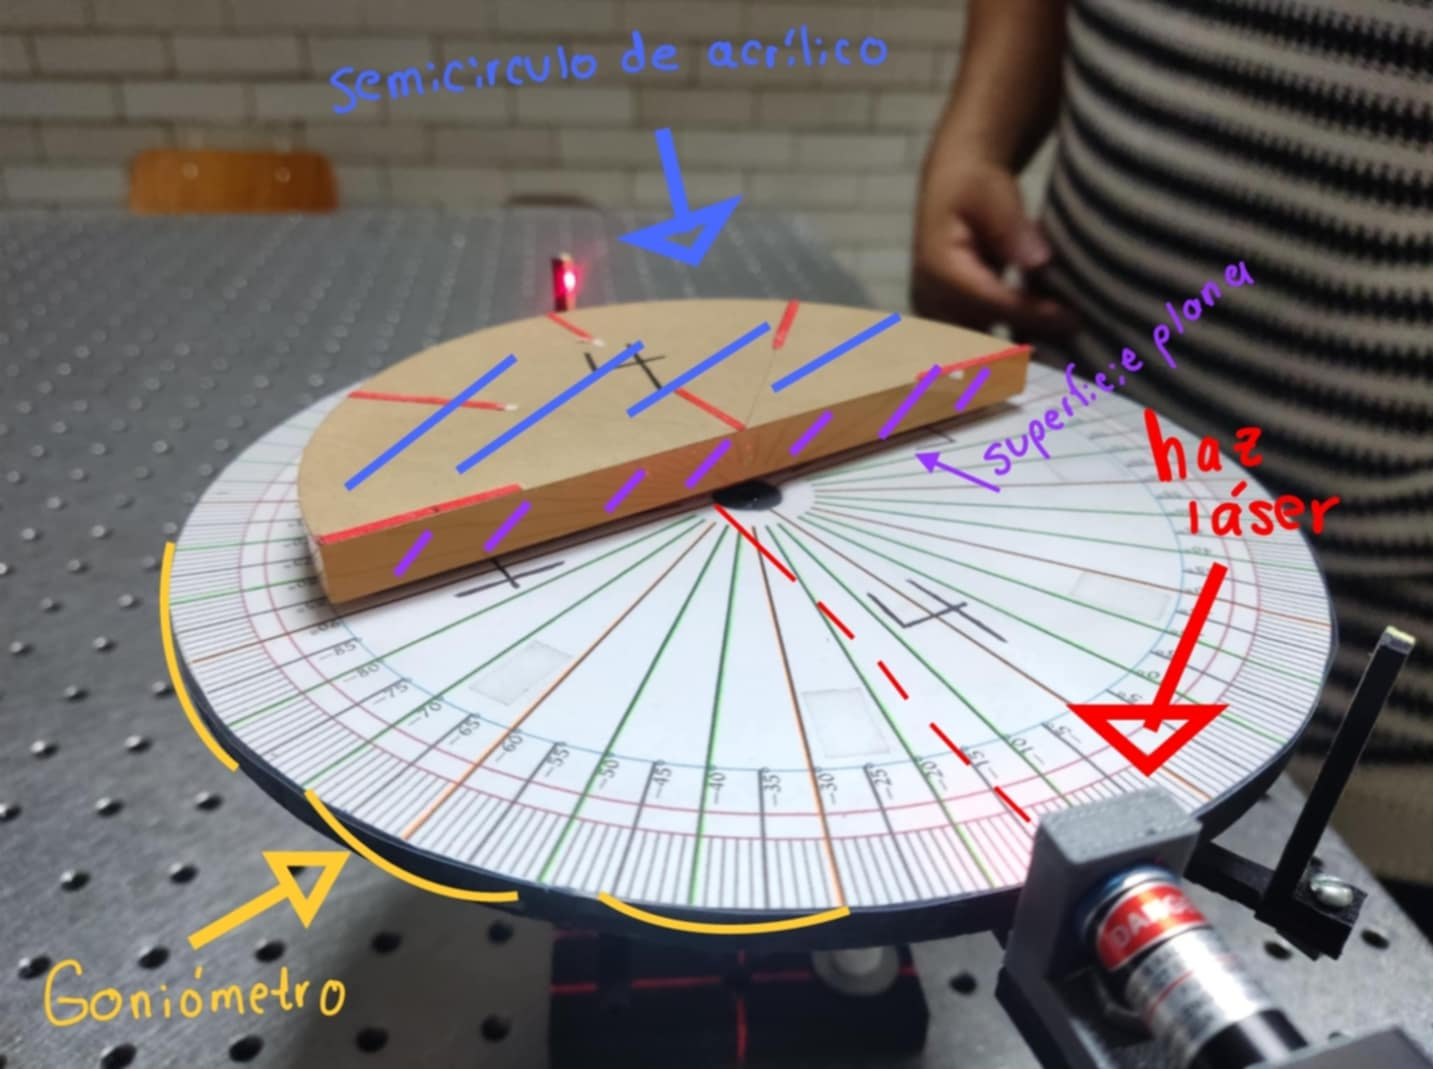
\includegraphics[width=0.5\linewidth]{arreglo experimental aire-acrílico.jpeg}
    \caption{Arreglo experimental Aire-Acrílico, fotografía por Ailton Reyes}
    \label{fig:enter-label}
\end{figure}

\subsection{Segunda parte: Incidencia en la cara circular (Acrílico-Aire)}
En la segunda parte del experimento, se dirigió el haz láser hacia la cara curva del bloque de acrílico. Este montaje permitió analizar el comportamiento de la luz al salir del medio denso hacia un medio menos denso y medir el ángulo crítico.

Los datos obtenidos del arreglo acrílico-aire fueron proporcionados por la dinámica grupal. A partir del análisis de las gráficas y los valores obtenidos, se calcularon la velocidad de la luz y el índice de refracción del acrílico. Como parte de este análisis, se propuso un nuevo objetivo: calcular el índice de refracción del acrílico utilizando la relación con el ángulo crítico de la reflexión interna total. 

\begin{figure}[H]
    \centering
    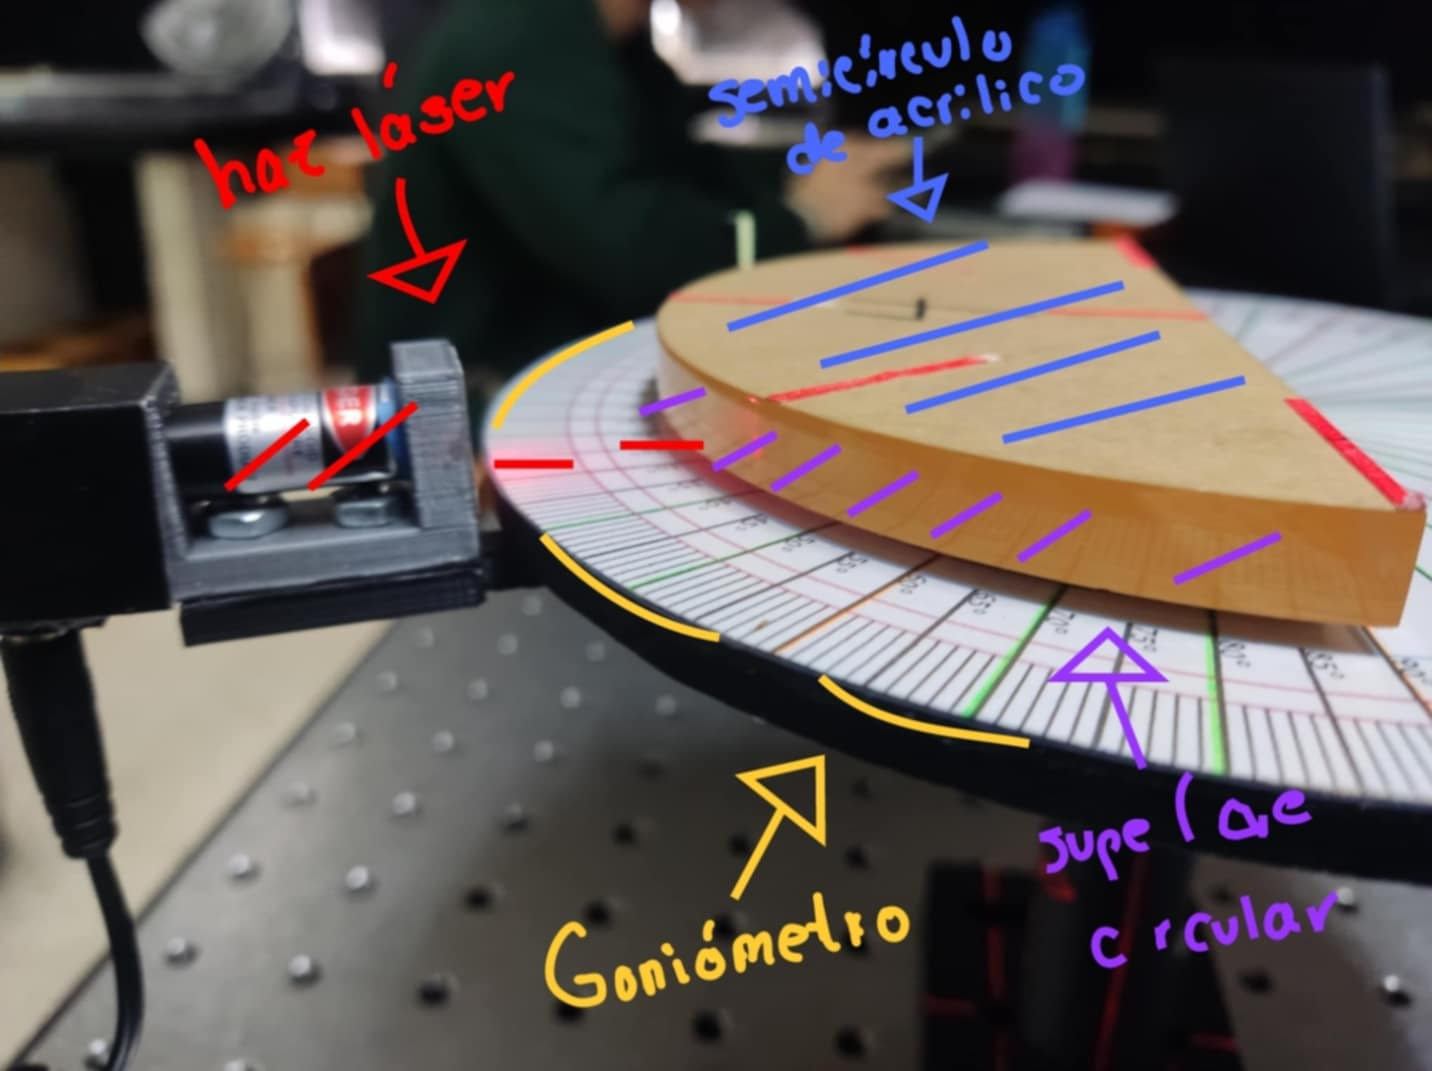
\includegraphics[width=0.5\linewidth]{arreglo experimental acrilico-aire.jpeg}
    \caption{Arreglo experimental Acrílico-Aire, fotografía por Ailton Reyes}
    \label{fig:enter-label}
\end{figure}

\subsection*{Tercera parte: Procedimiento para verificar n, a partir del ángulo crítico}
\begin{enumerate}
\item \textbf{Materiales necesarios}:
\begin{itemize}
\item Un bloque de material transparente (por ejemplo, vidrio o plástico) con superficies planas.
\item Un láser o fuente de luz monocromática.
\item Un transportador o sistema de medición angular.
\item Un soporte para ajustar el ángulo de incidencia.
\end{itemize}
\item \textbf{Montaje experimental}:
\begin{itemize}
    \item Coloca el bloque de material sobre una superficie plana.
    \item Dirige el haz de luz hacia una de las caras del bloque, variando el ángulo de incidencia ($\theta_I$).
    \item Observa el haz refractado y reflejado.
\end{itemize}

\item \textbf{Medición del ángulo crítico}:
\begin{itemize}
    \item Aumenta gradualmente el ángulo de incidencia ($\theta_I$) hasta que el haz refractado desaparezca y solo se observe el haz reflejado. Este ángulo es el \textbf{ángulo crítico} ($\theta_c$).
    \item Registra el valor de $\theta_c$.
\end{itemize}

\item \textbf{Cálculo del índice de refracción}:
\begin{itemize}
    \item Usa la ecuación derivada de la Ley de Snell para calcular el índice de refracción:
    \begin{equation}
    n = \frac{1}{\sin(\theta_c)}
    \end{equation}
\end{itemize}

\section{Resultados y tratamiento de datos}

\subsection{Aire-Acrílico}

Al registrar el ángulo de incidencia, ángulo de  reflexión y ángulo transmitido en el arreglo Aire-Acrílico se obtuvo la siguiente tabla (también puede consultar esta y las demás tablas en el enlace a hojas de cálculo de google \cite{Excel}):

\begin{table}[H]
\centering
\begin{tabular}{
>{\columncolor[HTML]{E2EFD9}}c 
>{\columncolor[HTML]{FEF2CB}}c 
>{\columncolor[HTML]{E2EFD9}}c 
>{\columncolor[HTML]{FEF2CB}}c 
>{\columncolor[HTML]{E2EFD9}}c 
>{\columncolor[HTML]{FEF2CB}}c 
>{\columncolor[HTML]{E2EFD9}}c 
>{\columncolor[HTML]{FEF2CB}}c 
>{\columncolor[HTML]{E2EFD9}}c 
>{\columncolor[HTML]{E2EFD9}}c }
\multicolumn{10}{c}{\cellcolor[HTML]{ECECEC}{\color[HTML]{2E75B5} \textbf{Aire - Acrílico}}} \\
\cellcolor[HTML]{92D050}\vartheta_I   (^{\circ}) &
  \cellcolor[HTML]{FFD965}\delta\vartheta_I   (^{\circ}) &
  \cellcolor[HTML]{92D050}\vartheta_R  (^{\circ}) &
  \cellcolor[HTML]{FFD965}\delta\vartheta_R   (^{\circ}) &
  \cellcolor[HTML]{92D050}\vartheta_T   (^{\circ}) &
  \cellcolor[HTML]{92D050}\delta\vartheta_T   (^{\circ}) &
  \cellcolor[HTML]{92D050}sin(\vartheta_I) _{rad} &
  \cellcolor[HTML]{FFD965}\deltasin(\vartheta_I) _{rad} &
  \cellcolor[HTML]{92D050}sin(\vartheta_T) _{rad} &
  \cellcolor[HTML]{FFD965}\delta sin(\vartheta_T) _{rad} \\
0     & 0.50    & 0     & 0.5    & 0       & 0.5    & 0.00    & 0.009    & 0.00    & 0.01    \\
5     & 0.5     & 5     & 0.5    & 3       & 0.5    & 0.09    & 0.009    & 0.05    & 0.01    \\
10    & 0.5     & 10    & 0.5    & 7       & 0.5    & 0.17    & 0.009    & 0.12    & 0.01    \\
15    & 0.5     & 15    & 0.5    & 10      & 0.5    & 0.26    & 0.009    & 0.17    & 0.01    \\
20    & 0.5     & 20    & 0.5    & 13      & 0.5    & 0.34    & 0.009    & 0.22    & 0.01    \\
25    & 0.5     & 25    & 0.5    & 16.5    & 0.5    & 0.42    & 0.009    & 0.28    & 0.01    \\
30    & 0.5     & 30    & 0.5    & 20      & 0.5    & 0.50    & 0.009    & 0.34    & 0.01    \\
35    & 0.5     & 35    & 0.5    & 23      & 0.5    & 0.57    & 0.009    & 0.39    & 0.01    \\
40    & 0.5     & 40    & 0.5    & 25      & 0.5    & 0.64    & 0.009    & 0.42    & 0.01    \\
45    & 0.5     & 45    & 0.5    & 29      & 0.5    & 0.71    & 0.009    & 0.48    & 0.01    \\
50    & 0.5     & 50    & 0.5    & 32.5    & 0.5    & 0.77    & 0.009    & 0.54    & 0.01    \\
55    & 0.5     & 55    & 0.5    & 34      & 0.5    & 0.82    & 0.009    & 0.56    & 0.01    \\
60    & 0.5     & 60    & 0.5    & 36      & 0.5    & 0.87    & 0.009    & 0.59    & 0.01    \\
65    & 0.5     & 65    & 0.5    & 38      & 0.5    & 0.91    & 0.009    & 0.62    & 0.01    \\
70    & 0.5     & 70    & 0.5    & 40      & 0.5    & 0.94    & 0.009    & 0.64    & 0.01    \\
75    & 0.5     & 75    & 0.5    & 41.5    & 0.5    & 0.97    & 0.009    & 0.66    & 0.01    \\
80    & 0.5     & 80    & 0.5    & 42      & 1.5    & 0.98    & 0.009    & 0.67    & 0.85    \\
85    & 0.5     & 85    & 0.5    & 43      & 1.5    & 1.00    & 0.009    & 0.68    & 0.85   
\end{tabular}
\caption{Ángulo de desviación de la luz del medio aire al acrílico}
\label{tab:my-table}
\end{table}

De la anterior tabla (Aire-Acrilico) podemos sacar su gráfica correspondiente, usando la ecuación linealizada de la reflexión (Ec. 2 del marco teórico)

\begin{figure}[H]
    \centering
    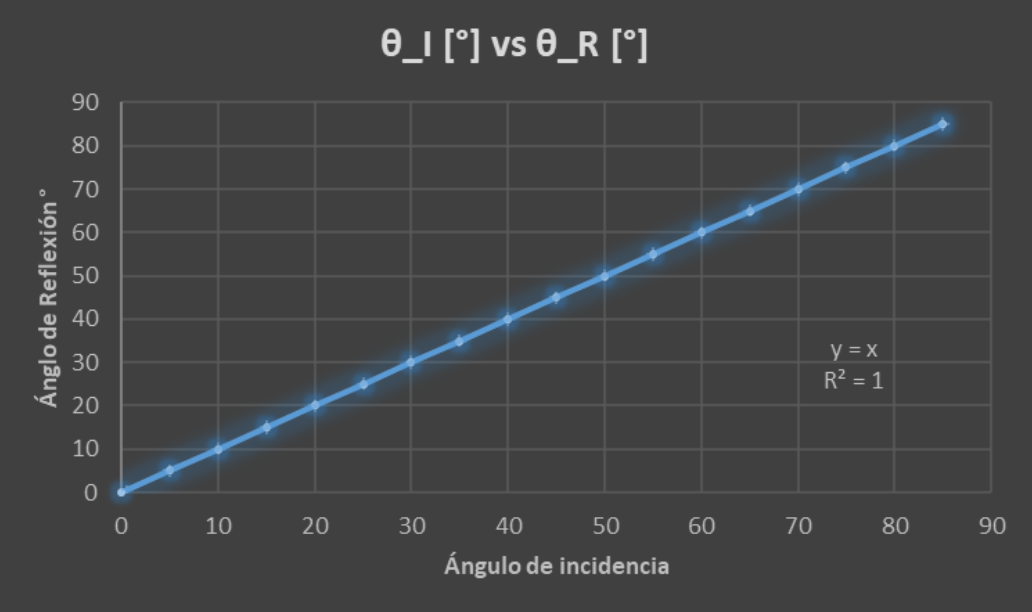
\includegraphics[width=0.5\linewidth]{Grafica 1 (aire-acrilico)).png}
    \caption{Gráfica de $\theta_I$ vs $\theta_R$ para aire-acrílico}
    \label{fig:enter-label}
\end{figure}

La pendiente de nuestra gráfica es $m=1$. Podemos comprobar ley de Snell (Ec. 4 del marco teórico) con los datos medidos en la tabla 1 (Aire-Acríilico) también podemos realizar la gráfica con la ecuación linealizada de la ley de Snell (Ec. 5 del marco teórico).

\begin{figure}[H]
    \centering
    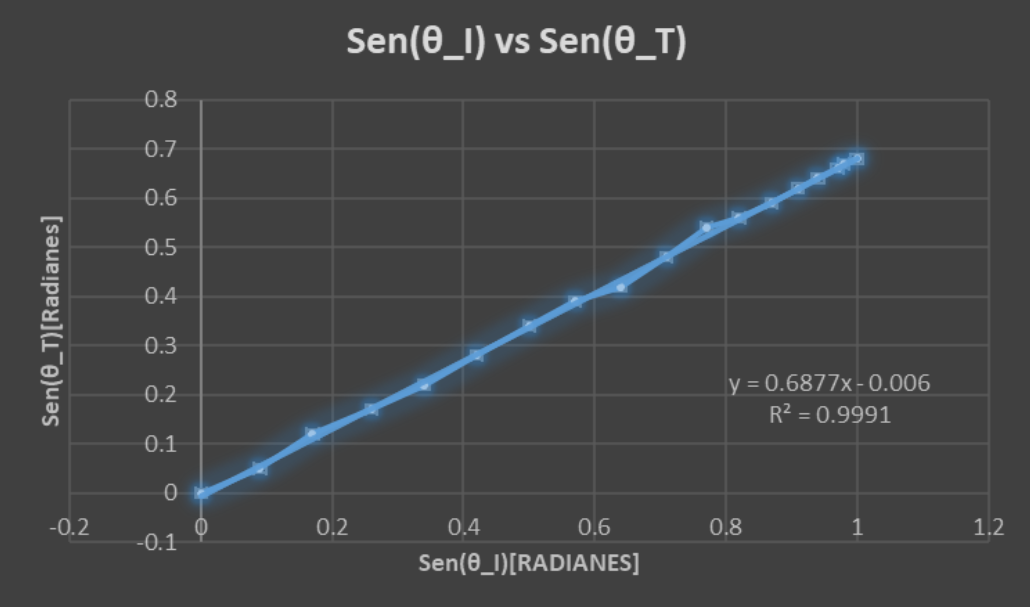
\includegraphics[width=0.5\linewidth]{Grafica 2 (aire-acrílico)).png}
    \caption{Gráfica sen$\theta_I$ vs sen$\theta_T$ para aire-acrílico}
    \label{fig:enter-label}
\end{figure}
La pendiente de la gráfica así como su incertidumbre estadística(obtenida con la función estamción lineal en excel) $m=0.6877\pm 0.0022$, además la incertidumbre de propagación asociada a está pendiente es $\pm$0.2367 la cual se obtiene a partir de la ecuación 13 del anexo. Por lo tanto la incertidumbre absoluta de m es $\pm$0.2367 así $m=0.6877 \pm 0.2367$  la cual es la suma en cuadratura de la incertidumbre estadística y la nominal.  
Ahora con esta pendiente  podemos calcular la velocidad del medio, multiplicando la pendiente por la velocidad de la luz. $m \cdot c= (0.6877\pm0.2367)\cdot(2.99792 \cdot 10^8\frac{m}{s})=V_m=\left(2.062\pm 0.3442\right)E+08 \frac{m}{s}$


\subsection{Acrílico-Aire (Datos del equipo 5)}

En la siguiente tabla se presentan los datos recopilados de otro equipo de laboratorio, de la misma forma que la sección pasada se midieron los mismos ángulos pero ahora incidiendo el haz a la superficie circular del acrílico semicírcular.

\begin{table}[H]
\centering
\begin{tabular}{
>{\columncolor[HTML]{E2EFD9}}c 
>{\columncolor[HTML]{FEF2CB}}c 
>{\columncolor[HTML]{E2EFD9}}c 
>{\columncolor[HTML]{FEF2CB}}c 
>{\columncolor[HTML]{E2EFD9}}c 
>{\columncolor[HTML]{FEF2CB}}c 
>{\columncolor[HTML]{E2EFD9}}c 
>{\columncolor[HTML]{E2EFD9}}c 
>{\columncolor[HTML]{E2EFD9}}c 
>{\columncolor[HTML]{E2EFD9}}c }
\multicolumn{10}{c}{\cellcolor[HTML]{ECECEC}{\color[HTML]{2E75B5} \textbf{Acrílico - Aire}}} \\
\cellcolor[HTML]{92D050}\vartheta_I   (^{\circ}) &
  \cellcolor[HTML]{FFD965}\delta\vartheta_I   (^{\circ}) &
  \cellcolor[HTML]{92D050}\vartheta_R  (^{\circ}) &
  \cellcolor[HTML]{FFD965}\delta\vartheta_R   (^{\circ}) &
  \cellcolor[HTML]{92D050}\vartheta_T   (^{\circ}) &
  \cellcolor[HTML]{92D050}\delta\vartheta_T   (^{\circ}) &
  \cellcolor[HTML]{92D050}sin(\vartheta_I)_{rad} &
  \cellcolor[HTML]{FFD965}\deltasin(\vartheta_I)_{rad} &
  \cellcolor[HTML]{92D050}sin(\vartheta_T)_{rad} &
  \cellcolor[HTML]{FFD965}\deltasin(\vartheta_T)_{rad} \\
4      & 0.5     & 3     & 0.5    & 5     & 0.5    & 0.07    & 0.009    & 0.09    & 0.009    \\
8      & 0.5     & 7     & 0.5    & 11    & 0.5    & 0.14    & 0.009    & 0.19    & 0.009    \\
12     & 0.5     & 11    & 0.5    & 16    & 0.5    & 0.21    & 0.009    & 0.28    & 0.008    \\
16     & 0.5     & 15    & 0.5    & 23    & 0.5    & 0.28    & 0.008    & 0.39    & 0.008    \\
20     & 0.5     & 19    & 0.5    & 30    & 0.5    & 0.34    & 0.008    & 0.50    & 0.008    \\
24     & 0.5     & 24    & 0.5    & 36    & 0.5    & 0.41    & 0.008    & 0.59    & 0.007    \\
28     & 0.5     & 28    & 0.5    & 44    & 0.5    & 0.47    & 0.008    & 0.69    & 0.006    \\
32     & 0.5     & 32    & 0.5    & 51    & 0.5    & 0.53    & 0.007    & 0.78    & 0.005    \\
36     & 0.5     & 35    & 0.5    & 60    & 0.5    & 0.59    & 0.007    & 0.87    & 0.004    \\
40     & 0.5     & 40    & 0.5    & 73    & 0.5    & 0.64    & 0.007    & 0.96    & 0.003    \\
2      & 0.5     & 1     & 0.5    & 2     & 0.5    & 0.03    & 0.009    & 0.03    & 0.009    \\
6      & 0.5     & 5     & 0.5    & 8     & 0.5    & 0.10    & 0.009    & 0.14    & 0.009    \\
10     & 0.5     & 10    & 0.5    & 14    & 0.5    & 0.17    & 0.009    & 0.24    & 0.008    \\
14     & 0.5     & 14    & 0.5    & 21    & 0.5    & 0.24    & 0.008    & 0.36    & 0.008    \\
18     & 0.5     & 17    & 0.5    & 26    & 0.5    & 0.31    & 0.008    & 0.44    & 0.008    \\
22     & 0.5     & 22    & 0.5    & 33    & 0.5    & 0.37    & 0.008    & 0.54    & 0.007    \\
26     & 0.5     & 26    & 0.5    & 39    & 0.5    & 0.44    & 0.008    & 0.63    & 0.007    \\
30     & 0.5     & 29    & 0.5    & 47    & 0.5    & 0.50    & 0.008    & 0.73    & 0.006   
\end{tabular}
\caption{Ángulo de desviación de la luz del medio acrílico al aire}
\label{tab:my-table}
\end{table}

De la anterior tabla \cite{Excel} podemos graficar $\theta_I$ vs $\theta_R$ con ayuda de la Ec.2 del marco teórico. 

\begin{figure}[H]
    \centering
    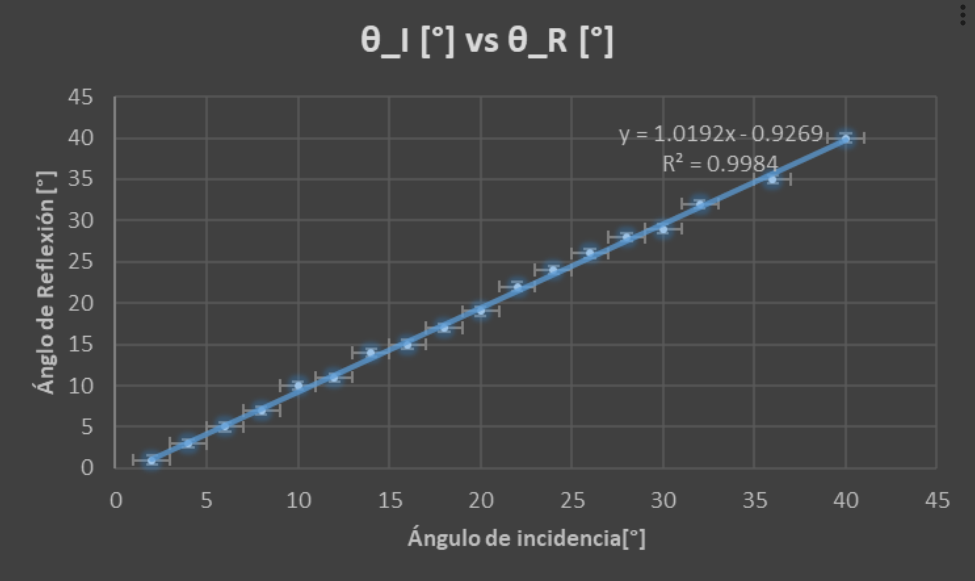
\includegraphics[width=0.5\linewidth]{Grafica1.1(acrílico-aire)).png}
    \caption{Gráfica $\theta_I$ vs $\theta_R$ para acrílico aire}
    \label{fig:enter-label}
\end{figure}

De la anterior gráfica obtenemos la pendiente así como su incertidumbre estádistica obtenida de la función estimación líneal de Excel $m=1.0192\pm 0.0103$ y además cuenta con una incertidumbre de propagación $\delta m = \pm 0.0240$ por lo que la incertidumbre obsoluta es $\Delta m = \pm 0.0275$ por lo tanto $m=1.0192 \pm 0.0275$, esta pendiente muestra un comportamiento similar a la teórica m=1 por lo que la ley de reflexión también se cumple en el arreglo acrílico-aire.

A contimuación analizaremos como en el caso pasado la ley de Snell, graficando gracias a la Ec.5 la cual es la linealización de la ley de Snell.

\begin{figure}[H]
    \centering
    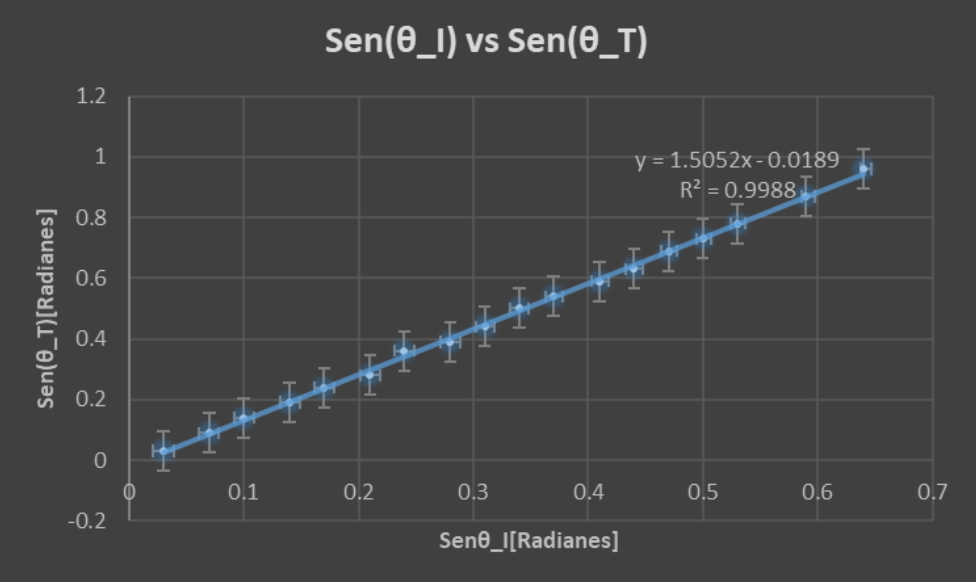
\includegraphics[width=0.5\linewidth]{Grafica 2.1(acrílico-aire)).png}
    \caption{Gráfica $sen(\theta_I)$vs$sen(\theta_T)$ para acrílico-aire}
    \label{fig:enter-label}
\end{figure}

Podemos observar el valor de la pendiente, así como su incertidumbre estadística calculada con la función de estimación lineal de excel $m=1.5052\pm 0.0099$ y cuya incertidumbre de propagación (Ec. 13) es $\pm$ 0.0642 así $\Delta m = \pm 0.0650$ por lo tanto $m = 1.5052 \pm 0.0650$.Con el valor de la pendiente podemos calcular la velocidad de la luz en el medio transmitido, esto es simplemente dividir entre la velocidad de la luz al índice de refracción obtenido como $m$ y calcular su inversa.

\begin{equation}
    v_{med} = \left( \frac{1.5052\pm 0.0650}{2.99792 \cdot 10^8} \right)^{-1} = \left(1.99170 \cdot  \pm 0.0432\right) \cdot 10^8 \frac{m}{s}
\end{equation}

Podmeos calcular el promedio de las pendientes en el caso de reflexión, para el arreglo aire-acrílico y acrílico-aire.

\[m_{promedio} = \frac{(m_1\pm \Delta m_1 )+(m_2 \pm \Delta m_2)}{2}= \frac{(1\pm0)+(1.0192\pm 0.0275)}{2}\]

\[m_{promedio}=1.0096\pm 0.0138 \]

Por otro lado podemos calcular el promedio de las velocidades en el caso de la refracción, para el arreglo aire-acrílico y acrílico aire

\[ v_{promedio}= \frac{(v_{m1}\pm \Delta v_{m1})+(v_{m2}\pm \Delta {v_2m})}{2}=\frac{(2.0628\pm 0.3442)\cdot 10^8+(1.99170\pm 0.0432 )\cdot10^8}{2}\]

\[v_{mpromedio}=\left(2.02725\cdot10^8\pm 0.19375\right)\cdot10^8\frac{m}{s}\]

\subsection{Índice de refracción a partir del ángulo crítico}

 Se encontró experimentalmente un angulo crítico $\theta_C=43^{\circ}\pm 0.5^{\circ}$ con este dato podemos calcular el índice de refrácción del medio(acrílico) utilizando la ecuación 7 del marco teórico, por otro lado calculamos la incertidumbre de n con la ecuación 13 que encontramos en el apartado del Anexo.

 \[n= \frac{1}{sen(\theta_C)}= \frac{1}{sen(43^{\circ})}= 1.46650\pm 0.39251\]

\section{Discusión de resultados}

\subsection{Reflexión y Refracción en la Interfaz Aire-Acrílico}
Los datos obtenidos en la Tabla \ref{tab:my-table} muestran que el ángulo de reflexión $\vartheta_R$ es aproximadamente igual al ángulo de incidencia $\vartheta_I$, lo que confirma la validez de la Ley de Reflexión con una incertidumbre mínima. La gráfica de $\vartheta_I$ vs. $\vartheta_R$ (Figura \ref{fig:enter-label}) presenta una pendiente de $m = 1.000 \pm 0.000$, lo que concuerda exactamente con la predicción teórica.

Por otro lado, la verificación de la Ley de Snell mediante la relación entre $\sin \vartheta_I$ y $\sin \vartheta_T$ muestra una pendiente de $m = 0.6877 \pm 0.2367$. Dado que esta pendiente es igual a la relación entre las velocidades de la luz en los dos medios ($v_{\text{acrílico}} / c$), se determinó la velocidad de la luz en el acrílico como:

\begin{equation}
V_{\text{acrílico}} = (2.062 \pm 0.344) \times 10^8 \text{ m/s}
\end{equation}

Este valor se encuentra dentro del orden de magnitud esperado para materiales poliméricos transparentes, aunque la incertidumbre relativa es del 16.7\%, lo que indica que la precisión del experimento podría mejorarse con mediciones de ángulos más precisas o con un láser de mayor coherencia espacial.

\subsection{Reflexión y Refracción en la Interfaz Acrílico-Aire}

Los datos obtenidos en la Tabla \ref{tab:my-table} para el experimento con incidencia desde el acrílico hacia el aire presentan una tendencia similar a la del caso aire-acrílico. La pendiente de la gráfica $\vartheta_I$ vs. $\vartheta_R$ es $m = 1.0192 \pm 0.0275$, lo que nuevamente verifica la Ley de Reflexión dentro de la incertidumbre experimental.

En cuanto a la Ley de Snell, la relación $\sin \vartheta_I$ vs. $\sin \vartheta_T$ dio una pendiente de $m = 1.5052 \pm 0.0650$, lo que corresponde al índice de refracción relativo entre el acrílico y el aire. A partir de este valor, se determinó la velocidad de la luz en el acrílico como:

\begin{equation}
V_{\text{acrílico}} = (1.9917 \pm 0.043) \times 10^8 \text{ m/s}
\end{equation}

Este resultado es consistente con el obtenido en la configuración aire-acrílico, con una menor incertidumbre relativa del 2.2\%, lo que indica que la medición en la configuración acrílico-aire fue más precisa.

Para cuantificar la concordancia entre los dos experimentos, se calculó el promedio de las velocidades obtenidas en ambas configuraciones:

\begin{equation}
V_{\text{acrílico, promedio}} = (2.027 \pm 0.194) \times 10^8 \text{ m/s}
\end{equation}

Este valor es coherente con referencias experimentales y valores reportados en la literatura para el acrílico ($\sim 2.0 \times 10^8$ m/s).$^6$

\subsection{Determinación del Índice de Refracción Mediante el Ángulo Crítico}

Se midió un ángulo crítico de $\theta_c = 43.0^\circ \pm 0.5^\circ$, a partir del cual se calculó el índice de refracción absoluto del acrílico mediante la ecuación:

\begin{equation}
n_{\text{acrílico}} = \frac{1}{\sin(43^\circ)} = 1.4665 \pm 0.3925
\end{equation}

El valor obtenido concuerda con el índice de refracción esperado para el acrílico ($n \approx 1.49$), aunque la incertidumbre es considerablemente alta (26.7\%). Esto puede deberse a la sensibilidad del método al error en la medición del ángulo crítico, ya que la derivada de la función $\sin^{-1}(\cdot)$ es relativamente grande en este rango angular.

\section{Conclusiones}

En este trabajo hemos verificado experimentalmente las leyes de reflexión y refracción mediante la incidencia de un haz láser en una interfaz aire-acrílico y acrílico-aire. A partir de mediciones angulares precisas, se confirmó que el ángulo de reflexión es igual al ángulo de incidencia, lo que valida empíricamente la Ley de Reflexión. Asimismo, la relación entre los senos de los ángulos de incidencia y refracción sigue la ecuación de Snell, lo que permitió determinar la velocidad de la luz en el acrílico y su índice de refracción.\\

El cálculo del índice de refracción a partir del ángulo crítico de reflexión interna total mostró un valor de $n = 1.4665 \pm 0.3925$, en concordancia con valores tabulados para materiales similares. Las incertidumbres fueron evaluadas rigurosamente mediante propagación de errores, lo que permitió cuantificar la precisión de nuestras mediciones y evaluar la fiabilidad de los resultados.\\

Este estudio refuerza el marco teórico de la óptica geométrica y demuestra la aplicabilidad de sus principios en la determinación de propiedades ópticas de materiales transparentes. Además, destaca la importancia de la propagación de incertidumbre en la obtención de resultados confiables. Futuros trabajos podrían explorar la dependencia del índice de refracción con la longitud de onda, o extender la metodología a otros materiales con diferentes propiedades ópticas.

 



\begin{thebibliography}{9}

\bibitem{Pedrotti2018} Pedrotti, F. L., Pedrotti, L. M., & Pedrotti, L. S. (2018). \textit{Introduction to Optics} (3\textsuperscript{a} ed.). Cambridge University Press.

\bibitem{Hecht2000} Hecht, E. (2000). \textit{Óptica} (3\textsuperscript{a} ed.). Addison Wesley.

\bibitem{Tipler1999} Tipler, P. A. (1999). \textit{Physics for Scientists and Engineers} (4\textsuperscript{a} ed.). Freeman/Worth.

\bibitem{Serway2002} Serway, R. A., & Beichner, R. J. (2002). \textit{Física para ciencias e ingeniería} (5\textsuperscript{a} ed.). McGraw-Hill.

\bibitem[]{Excel} A. Reyes, S. Tablas de Reflexión y Refracción, Archivo Excel. 2024. Descargar para ver la versión completa. \href{https://docs.google.com/spreadsheets/d/101YQkKrrlOy7PhZEOEiQAxeYIMbetz2N6dPFMMcdEuk/edit?usp=sharing}{https://docs.google.com/spreadsheets/d/101YQkKrrlOy7PhZEOEiQAxeYIMbetz2N6dPFMMcdEuk/edit?usp=sharing}

\bibitem{TESS2017} TESS Expert de PHYWE. (2017). \textit{Measuring the speed of light}. Physics.pub.ro. Recuperado el [fecha de acceso], de \href{http://www.physics.pub.ro/Cursuri/Electronica_I_G_(English)_2017/Laboratory_-_OPTICS/Measuring_the_speed_of_light.pdf}{http://www.physics.pub.ro/Cursuri/Electronica_I_G_(English)_2017/Laboratory_-_OPTICS/Measuring_the_speed_of_light.pdf}

\end{thebibliography}


\subsection*{Anexo}

\section*{Anexo: Propagación de Incertidumbre}
Para la pendiente $m$ en la Ley de Reflexión:

\begin{mdframed}
\begin{equation}
m = \frac{\theta_R}{\theta_I}
\end{equation}
\end{mdframed}

Aplicamos la propagación de incertidumbres:

\begin{mdframed}
\begin{equation}
\delta m= \sqrt{\left( \frac{\delta \theta_R}{\theta_R} \right)^2 + \left( \frac{\delta \theta_I}{\theta_I} \right)^2}
\end{equation}
\end{mdframed}

Para la Ley de Snell:

\begin{mdframed}
\begin{equation}
m = \frac{\sin \theta_T}{\sin \theta_I}
\end{equation}
\end{mdframed}

Aplicando la propagación de incertidumbres:

\begin{mdframed}
\begin{equation}
\delta m = \sqrt{\left( \frac{\cos \theta_T \cdot \delta \theta_T}{\sin \theta_T} \right)^2 + \left( \frac{\cos \theta_I \cdot \delta \theta_I}{\sin \theta_I} \right)^2}
\end{equation}
\end{mdframed}

Análisis de incertidumbres de ecuación 8

\begin{mdframed}
\begin{equation}
    \Delta n = \left| \frac{dn}{d\theta_c} \right| \cdot \Delta \theta_c = \left| -\frac{\cos(\theta_c)}{\sin^2(\theta_c)} \right| \cdot \Delta \theta_c
\end{equation}
\end{mdframed}

Incertidumbre propagada de la velocidad en el medio(acrílico)

\begin{mdframed}
\begin{equation}
\Delta V_m = \frac{\Delta m}{m}
\end{equation}
\end{mdframed}

\end{document}